\documentclass{article}
\usepackage{graphicx} % Required for inserting images

\usepackage{esint}
\title{Assignment 4}
\author{Sreeram Madhavan V\\Roll no: AE22B059\\Github Id: maxplankton}

\date{}
\begin{document}

\maketitle

\section*{AE22B059}
\section*{Assumptions}
\begin{figure}[h!]
    \centering
    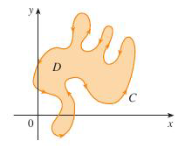
\includegraphics{Screenshot from 2023-06-18 01-03-52.png}
    \caption{This curve is in positive orientation}
    \label{fig:enter-label}
\end{figure}
C is a simple closed curve in X-Y plane.Positve orientation of C refers to a counterclockwise traversal of C.
\section*{Theorem}
\emph{Let C be a positively oriented simple closed piecewise smooth
curve in the plane. Let D be the region bounded by C. (That is, C = $\partial$D.) If M (x, y) and N (x, y)
have continuous partial derivatives on an open region containing D, then}\\\\
\begin{equation}
\oint_{C}Mdx+Ndy=\iint_{D}(\frac{\partial N}{\partial x}-\frac{\partial M}{\partial y})dA 
\end{equation}
\begin{equation}
\oint_{C}Mdy-Ndx=\iint_{D}(\frac{\partial N}{\partial y}+\frac{\partial M}{\partial x})dA
\end{equation} ~\cite{singh2022multivariable}
\section*{Application}

Green's Theorem provides the relationship between a simple closed curve C and the area enclosed D.
It can be used to analyse the surface D by choosing appropriate values for M and N. For example, Green's Theorem can be used as an effective tool to calculate the area enclosed by a curve. If we choose N=x and M=-y, we get:\\
\begin{equation}
\iint_{D}dA =\frac{1}{2}(\oint_{C}Mdy-Ndx)
\end{equation}\\
This is the area enclosed by C ~\cite{thomas1952calculus}
\section*{Reasons for choosing this topic }
Green's theorem has enormous application in physics and maths. It is useful in converting a line integral to surface integral or vice versa. Since I aspire to pursue theoretical physics in the future, this theorem seemed interesting to me.
\bibliographystyle{plain}
\bibliography{reference.bib}
\end{document}



